\documentclass[12pt, letterpaper, preprint]{aastex}
\usepackage[breaklinks,colorlinks, urlcolor=blue,citecolor=blue,linkcolor=blue]{hyperref}
\usepackage{hyperref}
\usepackage{color}
%%% This file is generated by the Makefile.
\newcommand{\giturl}{\url{https://github.com/changhoonhahn/centralMS}}
\newcommand{\githash}{9119283}\newcommand{\gitdate}{2019-04-05}\newcommand{\gitauthor}{changhoonhahn}


% typesetting shih
\linespread{1.08} % close to 10/13 spacing
\setlength{\parindent}{1.08\baselineskip} % Bringhurst
\setlength{\parskip}{0ex}
\let\oldbibliography\thebibliography % killin' me.
\renewcommand{\thebibliography}[1]{%
  \oldbibliography{#1}%
  \setlength{\itemsep}{0pt}%
  \setlength{\parsep}{0pt}%
  \setlength{\parskip}{0pt}%
  \setlength{\bibsep}{0ex}
  \raggedright
}
\setlength{\footnotesep}{0ex} % seriously?

\newcommand\tab[1][1cm]{\hspace*{#1}}
\newcommand{\todo}[1]{{\bf \textcolor{red}{#1}}}
\newcommand{\beq}{\begin{equation}}
\newcommand{\eeq}{\end{equation}}
\newcommand{\overbar}[1]{\mkern 1.5mu\overline{\mkern-1.5mu#1\mkern-1.5mu}\mkern 1.5mu}
\newcommand{\avgSFR}{\overline{\raisebox{0pt}[1.2\height]{SFR}}}
\newcommand{\SFR}{\mathrm{SFR}}
\newcommand{\fq}{f_\mathrm{Q}}
\newcommand{\fqcen}{f_\mathrm{Q}^\mathrm{cen}}
\newcommand{\zinit}{z_\mathrm{initial}}
\newcommand{\taucen}{\tau_\mathrm{Q}^\mathrm{cen}}
\newcommand{\logsfr}{\log \, \mathrm{SFR}}
\newcommand{\bitem}{\begin{itemize}}
\newcommand{\eitem}{\end{itemize}}
\newcommand{\musfms}{\log\,\overline{\mathrm{SFR}}_\mathrm{SFS}}
\newcommand{\siglogm}{\sigma_{\log\,M_*}} 
\newcommand{\hahngmm}{Hahn et al. (in prep.)} 

\begin{document}\sloppy\sloppypar\frenchspacing

\title{Star Formation Main Sequence in a Hierarchical Universe} 
%\title{Central Galaxies on the Main Sequence} 
\date{\texttt{DRAFT~---~\githash~---~\gitdate~---~NOT READY FOR DISTRIBUTION}}
\author{ChangHoon~Hahn\altaffilmark{1, 2}, 
Jeremy L.~Tinker\altaffilmark{2}, 
Andrew R.~Wetzel\altaffilmark{3,4,5}}
\altaffiltext{1}{Lawrence Berkeley National Laboratory, 1 Cyclotron Road, Berkeley, CA 94720}
\altaffiltext{2}{Center for Cosmology and Particle Physics, Department of Physics, New York University, 4 Washington Place, New York, NY 10003}
\altaffiltext{3}{TAPIR, California Institute of Technology, Pasadena, CA USA}
\altaffiltext{4}{Carnegie Observatories, Pasadena, CA USA}
\altaffiltext{5}{Department of Physics, University of California, Davis, CA USA}
\email{changhoon.hahn@lbl.gov}

\begin{abstract}
    \todo{motivation, methodology, impact.}
    In observations star forming galaxies form a tight $log\;M_*$ to $log\;SFR$ 
    relation referred to as the {\em star formation main sequence} (SFS) out to $z\sim2$. 
    Beyond the evolution ``along'' this SFS, however, the star formation histories of star 
    forming galaxies have not been precisely characterized. 
    The SFH of these galaxies govern SMF, SFS, and also observed constraints on the stellar mass to halo mass
    relation. 

    By combining high-resolution cosmological $N$-body simulation with observed evolutionary 
    trends of SF galaxies, we construct a model that tracks the evolution of star forming 
    central galaxies over the redshift $z < 1$. Comparing this model 

    Observations find a remarkably small scatter in the stellar mass to halo mass relation. 
    Somehow the star formation histories of galaxies must 
    
    According to observations, star forming galaxies form a tight $log\;M_*$ to $log\;SFR$ 
    relation referred to as the ``star formation main sequence'' out to $z\sim2$. 
\end{abstract}
\keywords{methods: numerical -- galaxies: clusters: general -- 
galaxies: groups: general -- galaxies: evolution -- galaxies: haloes -- 
galaxies: star formation -- cosmology: observations.}

\section{Introduction}
\bitem 
\item Motivate why we think SF galaxies evolve along the main sequence  
\item Discuss the current thought process on galaxy assembly bias 
\item Explain the limitation of SFH derivable from observations (Claire's fisher matrix paper would be really good; ask her about the details) 
\item Observations also can't provide detail host dark matter halo properties
\item So the approach with combining observations with N-body (empirical modeling) is very effective in the context of the halo.
\item Maybe talk about how the bigger context of why this is important?  
\item Why only centrals -- because our current best understanding of satellites is that they quench after infall, so it doesn't make sense to look at them
\item our model goes from $z < 1$ because beyond that the observations are statistically meaningless.  
\eitem 

%%%%%%%%%%%%%%%%%%%%%%%%%%%%%%%%%%%%%
% Figure 1 
%%%%%%%%%%%%%%%%%%%%%%%%%%%%%%%%%%%%%
\begin{figure}
\begin{center}
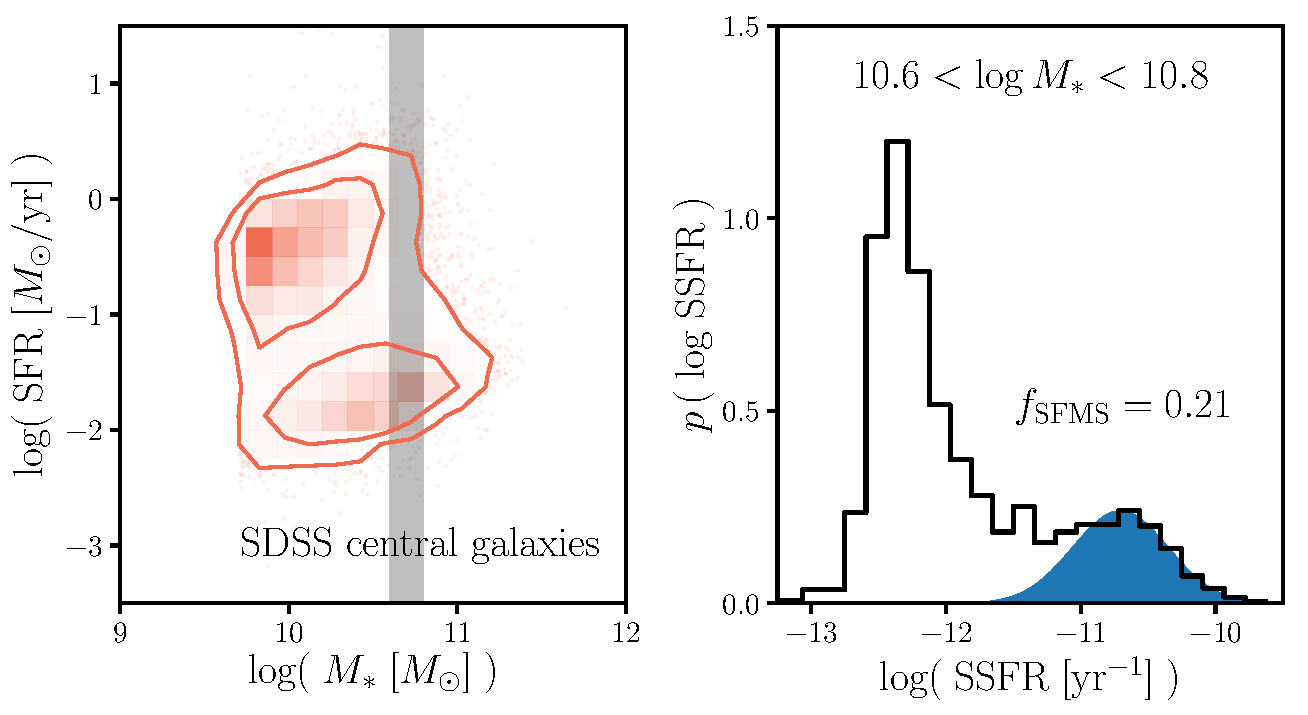
\includegraphics[width=0.9\textwidth]{figs/groupcat.pdf}
    \caption{Central galaxies of the SDSS DR7 group catalog. \emph{Left:} We plot 
    the SFR-$M_*$ relation of the SDSS central galaxies. The contours illustrate the bimodal
    distribution of the galaxy properties and mark the star-forming and quiescent populations. 
    The transitioning galaxies lie on the ``green'' valley between the star-fomring and quiescent
    modes. %The dashed line represents the linear fit to the SFS as described in Section~\ref{sec:sfcen}. 
    \emph{Right:} We plot the distribution of $\mathrm{log}\,\mathrm{SSFR}$ for SDSS centrals
    with $10.6 < \mathrm{log}\,M_* < 10.8$. Shaded in blue, we plot the SFS component of our 
    GMM fit of the SFR-$M_*$ relation described in Section~\ref{sec:sfcen}. Based on this fit, 
    galaxies in the SFS account for approximately $f_\mathrm{SFS} = 0.21$ of the central 
    galaxies in the stellar mass bin.} \label{fig:groupcat}
\end{center}
\end{figure}
%%%%%%%%%%%%%%%%%%%%%%%%%%%%%%%%%%%%%

\section{Central Galaxies of SDSS DR7} \label{sec:sdss}
We construct our galaxy sample following the sample selection of \cite{tinker2011}. 
We select a volume-limited sample of galaxies with $M_r −5 log(h) < −18$ and complete in
$M_* > 10^{9.4} M_\odot$ from the NYU Value-Added Galaxy Catalog \citep[VAGC;][]{blanton2005}
of the Sloan Digital Sky Survey Data Release 7~\citep[SDSS DR7;][]{abazajian2009} at 
$z \approx 0.04$. The stellar masses of these galaxies are estimated using the
$\mathtt{kcorrect}$ code~\citep{blanton2007} assuming a~\cite{chabrier2003} initial
mass function. The star formation of the galaxies are estimated spectroscopically using the
specific star formation rates (SSFR) from the current release of the MPA-JHU spectral 
reductions\footnote{http://wwwmpa.mpa-garching.mpg.de/SDSS/DR7/}~\citep{brinchmann2004}.
Generally speaking, $\mathrm{SSFR} > 10^{-11}\mathrm{yr}^{-1}$ are derived from 
$\mathrm{H}_\alpha$ emission, $10^{-11} > \mathrm{SSFR} > 10^{-12}\mathrm{yr}^{-1}$
are derived from a combination of emission lines, and $\mathrm{SSFR} < 10^{-12}\mathrm{yr}^{-1}$
are based on $D_n 4000$~\citep[see discussion in][]{wetzel2013}. We note that 
$\mathrm{SSFR} < 10^{-12}\mathrm{yr}^{-1}$ should only be considered upper limits 
to the true galaxy SSFR~\citep{salim2007}.

From our galaxy sample, we identify the central galaxies using the \cite{tinker2011} halo-based 
group-finding algorithm, which is based on the~\cite{yang2005} algorithm and tested 
in~\cite{campbell2015}. The algorithm assigns a probability of being a satellite,
$P_\mathrm{sat}$, to each galaxy in the sample. Galaxies with $P_\mathrm{sat} \geq 0.5$ 
are classified as satellites and $P_\mathrm{sat} < 0.5$ are classified as centrals. 
In this paper we focus on central galaxies. With any group finding algorithm, galaxies are 
misassigned due to projection effects and redshift space distortions. The purity 
of the full central galaxy sample is $\sim 90\%$ with a completeness of $\sim 95\%$~\citep{tinker2017}.
Furthermore, \cite{campbell2015} find that the algorithm robustly identifies red and blue centrals
as a function of stellar mass, which is highly relevant to our analysis.  

In the left panel of Figure~\ref{fig:groupcat}, we plot the SFR-$M_*$ distribution of
the SDSS DR7 central galaxies. In the right panel, we plot the distribution of SSFR, 
$p(\log \mathrm{SSFR})$, for galaxies with $10.6 < \log \,M_* < 10.8$ (stellar mass range 
highlighted on the left panel). Both panels of Figure~\ref{fig:groupcat} illustrate the 
bimodality in the galaxy sample. The SFR-$M_*$ distribution also illustrate the correlation
between SFR and $M_*$ in star-forming galaxies \emph{i.e.} the star-formation main sequence 
(SFS).

\section{Model: Simulated Central Galaxies} \label{sec:sim}
We're interesting in constructing a model that tracks central galaxies and 
their star formation within the heirarchical growth of their host halos. This 
requires a cosmological $N$-body simulation that accounts for the complex 
dynamical processes that govern the host halos of galaxies. In this paper 
we use the high resolution $N$-body simulation from~\cite{wetzel2013} generated 
using the \cite{white2002} $\mathtt{TreePM}$ code with flat $\Lambda$CDM cosmology 
($\Omega_m =0.274, \Omega_b = 0.0457, h = 0.7, n=0.95, \mathrm{and} \sigma_8 = 0.8$).
From initial conditions at $z = 150$ generated from second-order Lagrangian 
Perturbation Theory, $2048^3$ particles with mass of $1.98 \times 10^8\,M_\odot$ are 
evolved in a $250 \mathrm{Mpc}/h$ box with a Plummer equivalent smoothing of 
$2.5\,\mathrm{kpc}/h$. For a more detailed description of the simulation, we 
refer readers to~\cite{wetzel2013, wetzel2014}.

From the $\mathrm{TreePM}$ $N$-body simulation, `host halos' are identified 
using the Friends-of-Friends (FoF) algorithm of \cite{davis1985} with 
linking length of $b = 0.168$ times the mean inter-partcile spacing. Within 
these host halos, \cite{wetzel2013} identifies `subhalos' as overdensities 
in phase space through a six-dimensional FoF algorithm~\citep[FoF6D][]{white2010}. 
The host halos and subhalos are then tracked across the $45$ simulation 
outputs from $z = 10$ to $0$ to build merger trees~\citep{wetzel2009,wetzel2010}. 
The most massive subhalos in newly-formed host halos at a given simulation 
output are defined as the `central' subhalo. A central subhalo retains its 
`central' definition until it falls into a more massive host halo, at which 
point it becomes a `satellite' subhalo. 

Each subhalo is assigned a $M_\mathrm{peak}$, the maxmum host halo mass that 
it ever had as a central subhalo. Using $M_\mathrm{peak}$, we construct a galaxy 
catalog from the subhalos using subhalo abundance 
matching~\citep[SHAM;][]{conroy2006,vale2006,yang2009,wetzel2012,leja2013,wetzel2013,wetzel2014,hahn2017a}. 
In principle, SHAM assumes a one-to-one mapping between subhalo 
$M_\mathrm{peak}$ and galaxy stellar mass $M_*$: $n(> M_\mathrm{peak}) > n(> M_*)$
that preserves the rank ordering. In practice, we apply a $0.2$ dex log-normal 
scatter in $M_∗$ at fixed $M_\mathrm{peak}$ based on observations of the stellar 
mass to halo mass relation (SMHMR; \todo{bunch of SMHMR citations}). \cite{gu2016} 
compile empirical constraints on the scatter of this stellar mass to halo 
mass relation ($\sigma_{\log M_*}$). Using the SHAM mapping, we can 
assign galaxy stellar mass to subhalos based on observed stellar mass 
functions (SMFs) at the redshifts of the simulation outputs (snapshots). 

We use the SMF from \cite{li2009} at $z = 0.05$ and at higher redshifts 
interpolate between the \cite{li2009} SMF and the SMF from \cite{marchesini2009} 
at $z = 1.6$. We choose the \cite{li2009} SMF because it is based on the 
same SDSS NYU-VAGC sample as our SDSS DR7 group catalog (Section~\ref{sec:sdss}). 
We choose the \cite{marchesini2009} SMF, amongst others, because it produces 
interpolated SMFs that monotonically increase at $z < 1$. As noted in 
\cite{hahn2017a}, at $z \approx 1$, the SMF interpolated between the 
\cite{li2009} and \cite{marchesini2009} SMFs is consistent with more 
recent measurements from \cite{muzzin2013} and \cite{ilbert2013}. 
At each snapshot, we independently use SHAM to assign galaxy $M_*$. 
This way, we not only track the evolution of subhalos, but also the 
the galaxies' $M_*$. With the $45$ snapshots outputs from our simulation, 
we can in principle track the central galaxies back to $z \sim 10$. 
However, we restrict ourselves to snapshots at $z \lesssim 1$, where we 
have the most statistically meaningful observations. We next describe
how we select star forming central galaxies in our model and initalize them. 
%As we desribe later in this section, however, we're only interested in the snapshots at $z \approx 0.05$ and $1$, respectively. 
\todo{TBD: Perhaps mention in appendix how we test different SMF assumptions}% (In Section~\ref{app:z1},)

%%%%%%%%%%%%%%%%%%%%%%%%%%%%%%%%%%%%%
% Figure 2 
%%%%%%%%%%%%%%%%%%%%%%%%%%%%%%%%%%%%%
%\begin{figure}
%\begin{center}
%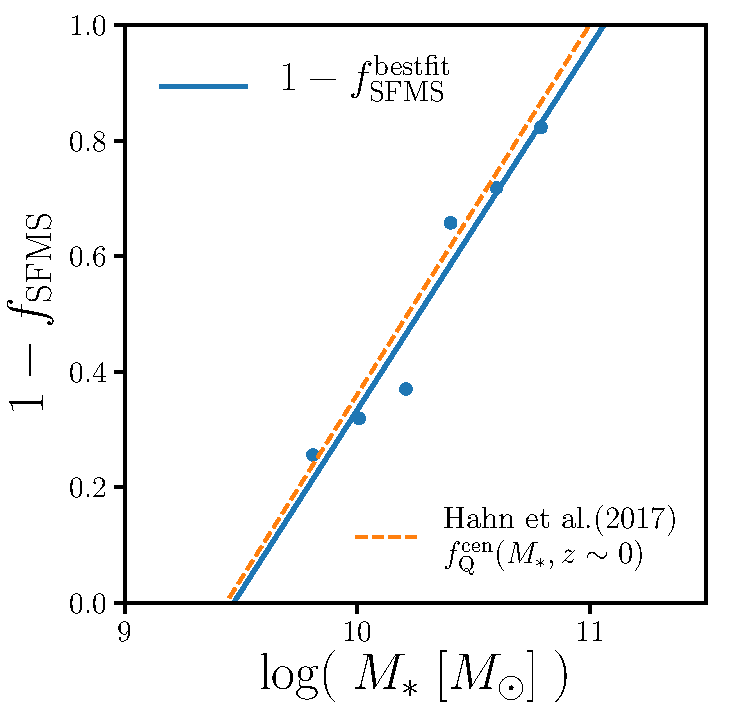
\includegraphics[width=0.5\textwidth]{figs/fq_fsfms.pdf}
%\caption{SFS fraction versus quiescent fraction from Hahn}
%\label{fig:fq_fsfms}
%\end{center}
%\end{figure}
%%%%%%%%%%%%%%%%%%%%%%%%%%%%%%%%%%%%%

\subsection{Selecting Star Forming Centrals}  \label{sec:sfcen}
In our model, we're interested in tracking the SFR and stellar mass 
evolution of SF central galaxies. To construct such a model, we 
first need to select SF galaxies from the central galaxies in our 
simulation, described above. Since we want our model to reproduce 
observations, our selection is based on $f^\mathrm{cen}_\mathrm{SFS}(M_*)$, 
the fraction of central galaxies within the star forming sequence, 
measured from the SDSS DR7 VAGC (Section~\ref{sec:sdss}). Below, we 
describe how we derive this $f^\mathrm{cen}_\mathrm{SFS}(M_*)$ and use 
it to select SF central galaxies in our model. Afterwards we describe how 
we initalize the SFRs and $M_*$ of these galaxies in our model.

Often in the literature, an empirical color-color or SFR--$M_*$ cut 
that separates the two main modes (red/blue or star-forming/quiescent) 
in the distribution is chosen to classify 
galaxies~\citep[\emph{e.g.}][]{baldry2006, blanton2009, drory2009, peng2010, moustakas2013, hahn2015}.
The red/quiescent or blue/star-forming fractions derived from this sort 
of classification, by construction, depend on the choice of cut and 
neglect galaxy subpopulations such as transitioning galaxies~\emph{i.e.} 
galaxies in the ``green valley''. Instead, for our 
$f^\mathrm{cen}_\mathrm{SFS}(M_*)$, we use the SFS fitting method 
from \hahngmm. \hahngmm uses Gaussian Mixture Models and the Bayesian 
Information Criteria in order to fit the SFR--$M_*$ relation of a galaxy 
population and identify its SFS. This data-driven approach relaxes 
many of the assumptions and hard cuts that go into other methods. 
Furthermore, as they demonstrate in \hahngmm by applying to multiple 
simulations, it can be flexibly applied to a wide range of star 
formation and $M_*$. The weight of the SFS GMM component from the 
fitting provides an estimate of $f^\mathrm{cen}_\mathrm{SFS}$. 
In the right panel of Figure~\ref{fig:groupcat}, we plot the SFS 
GMM component (blue shaded region) of the $p(\log \mathrm{SSFR})$ 
for the SDSS DR7 central galaxies within $10.6 < \log M_* < 10.8$. 
The SFS constitutes $f^\mathrm{cen}_\mathrm{SFS} = 0.21$ of the 
SDSS central galaxies in this stellar mass bin. 

%we instead use a method from \todo{Hahn et al.~(in prep)} and Tjitske et 
%al.~(in prep), which is a data-driven fitting of the SFS from the SFR-$M_*$ 
%distribution using Gaussian Mixture Models (GMMs). 
%Using the Hahn et al.~(in prep) SFS fitting, we fit the SSFR 
%distributions of the SDSS DR7 VAGC centrals in $\log\,M_*$ bins 
%of width $0.2~\mathrm{dex}$ using GMMs with $k = 1 - 3$ components 
%using the expectation-maximization 
%algorithm~\citep[EM;][]{dempster1977, neal1998}. We restrict 
%ourselves to models with a maximum of $3$ components for the three 
%possible galaxy classifications: quiescent, SF, and transitioning populations. From the three GMMs, we select the model with 
%the lowest Bayesian Information Criteria~\citep[BIC;][]{schwarz1978}. 
%The Gaussian component of this GMM with mean $\log \mathrm{SSFR} > -11$ 
%is identified as the SFS. In the rare cases when more than one GMM 
%component has mean $\log \mathrm{SSFR} > -11$, we compare the weights 
%of the components.  If the weight of one component is less than a 
%third of the other, we take the component with the higher weight to 
%represent the SFS. Otherwise, we omit the stellar mass bin altogether. 
%\todo{sentence about how for the VAGC, we don't omit any stellar mass bins} 

Rather than using the $f^\mathrm{cen}_\mathrm{SFS}$ values directly, 
for selecting SF galaxies, we fit $f^\mathrm{cen}_\mathrm{SFS}$ as 
a linear function of $\log\,M_*$ similar to \cite{wetzel2013,hahn2017}. 
We derive the following best-fit: 
\beq \label{eq:f_cen_sfms}
f^\mathrm{cen}_\mathrm{SFS, bestfit}(M_*) = -0.627\,(\log\,M_* - 10.5) + 0.354. 
\eeq
We note that this $f^\mathrm{cen}_\mathrm{SFS, bestfit}(M_*)$ is in good 
agreement with the $f_\mathrm{Q}^\mathrm{cen}(M_*; z\sim0)$ fit from 
\cite{hahn2017a}. For each central galaxy in our simulation, we assign 
a probability of it being on the SFS, using Eq.~\ref{eq:f_cen_sfms} 
with $M_*$ at $z \sim 0$ assigned through SHAM. Based on these 
probablities, we randomly identify centrals from our simulation as SF at 
$z \sim 0$. In our model, we make the assumption that once a SF galaxy 
quenches its star formation, it remains quiescent.  %\todo{maybe something about rejuvenation?} 
Without any quiescent galaxies rejuvenating their star formation, galaxies
on the SFS at $z\sim0$ are also on the SFS at $z > 0$. Using this assumption
the SF centrals we select at $z \sim 0$ are also on the SFS at the intial
redshift of our model: $z \sim 1$. 

Next, we can initialize the SF centrals at $z\sim1$ using SHAM $M_*$s and 
assign their initial SFRs based on the observed SFR-$M_*$ relation of the SFS. 
Observations in the literature at these redshifts, however, not only use 
galaxy properties derived differently from the SDSS VAGC but they also 
find SFS with significant discrepancies from one another. \cite{speagle2014} 
compiles the SFR-$M_*$ relation of the SFS from 25 studies in the literature, 
each with different methods of deriving galaxy properties. Even \emph{after} 
their calibration, for a fixed $M_* = 10^{10.5}\, M_\odot$, the SFRs of the 
SFSs at $z \sim 1$ vary by more than a factor of 2~\citep[see Figure 2 of][]{speagle2014}. 
With little consensus on the SFS at $z\sim1$, and consequently its redshift
evolution, we flexibly parameterize the SFS SFR ($\log\,\mathrm{SFR}_\mathrm{MS}(M_*, z)$) 
with free parameters $m_{M_*}$ and $m_z$ that characterize the stellar mass 
and redshift dependences respectively.  %and marginalize over them later in the analysis. 
%This is particularly concerning since the redshift evolution of the SFS dictate the SFR and $M_*$ evolution of SF centrals in our model. 
%So to deal with this uncertainty, we parameterize 
%For our $\log\,\mathrm{SFR}_\mathrm{MS}(M_*, z)$, at $z \sim 0$ we anchor our 
%SFS to the SFS of the SDSS central galaxies, which we obtain from the 
%SFS GMM components used to estimate $f^\mathrm{cen}_\mathrm{SFS}$. Using 
%the mean $\log\, \mathrm{SFR}$ of the SFS GMM component at each stellar 
%mass bin, we linearly fit $\log\, \mathrm{SFR}(M_*)$ (see dashed line in 
%Figure~\ref{fig:groupcat}). Then for $z > 0$, we include two free 
%parameters to account for the redshift evolution of the amplitude and 
%slope of the SFS SFR-$M_*$ relation: $A_z$ and $m_z$, respectively. 
We parameterize the mean $\log\,\mathrm{SFR}$ of the SFS as, 
\beq \label{eq:logsfr_ms}
\log\,\overline{\mathrm{SFR}}_\mathrm{SFS}(M_*, z) =  m_{M_*} * (\log\,M_* - 10.5) + m_z * (z - 0.05) - 0.11.
\eeq
We assign SFRs to our SF centrals at $z\sim1$ by sampling a log-normal 
distribution centered about $\log\,\overline{\mathrm{SFR}}_\mathrm{MS}(M_*, z=1)$ 
with a constant scatter of $0.3\,\mathrm{dex}$, motivated from 
observations~\citep{daddi2007, noeske2007, magdis2012, whitaker2012}.
Later in our analysis, for the priors of our parameters $m_{M_*}$ 
and $m_z$, we conservatively choose a range that encompass the best-fit 
SFS from~\cite{speagle2014} and measurements from~\cite{moustakas2013} 
and~\cite{lee2015}. With our SF centrals initalized at $z \sim 1$, next, 
we describe how we evolve their SFR and $M_*$.

%%%%%%%%%%%%%%%%%%%%%%%%%%%%%%%%%%%%%
% Figure 3 
%%%%%%%%%%%%%%%%%%%%%%%%%%%%%%%%%%%%%
\begin{figure}
\begin{center}
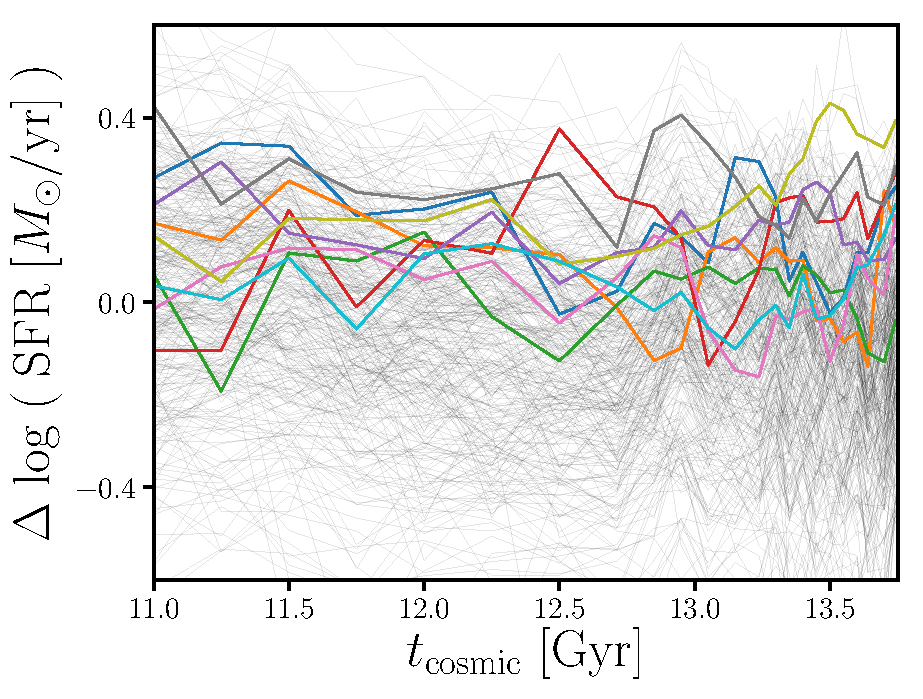
\includegraphics[width=0.5\textwidth]{figs/illustris_sfh.pdf} 
    \caption{Star formation rate with respect to the $\musfms$---$\Delta \logsfr$)---as 
    a function of cosmic time for star-forming galaxies in the Illustris simulation. 
    These galaxies have stellar masses within the range $10^{10.5}-10^{10.6}M_\odot$ 
    at $z\sim0$. $\musfms$ is fit using the \hahngmm SFS fitting method, the same method
    we use for our SDSS centrals in Section~\ref{sec:sfcen}. As the $\Delta \logsfr(t)$s
    in color emphasize how the SFRs of Illustris star-forming galaxies fluctuate about 
    the mean SFS. \emph{The $\mathrm{SFR}$ variability in the SFHs of SF centrals in our model (see 
    Section~\ref{sec:modelevol}) is motivated by this $\Delta \logsfr(t)$ behavior in 
    Illustris.}}
\label{fig:illsfh}
\end{center}
\end{figure}
%%%%%%%%%%%%%%%%%%%%%%%%%%%%%%%%%%%%%

%%%%%%%%%%%%%%%%%%%%%%%%%%%%%%%%%%%%%
% Figure 4 
%%%%%%%%%%%%%%%%%%%%%%%%%%%%%%%%%%%%%
\begin{figure}
\begin{center}
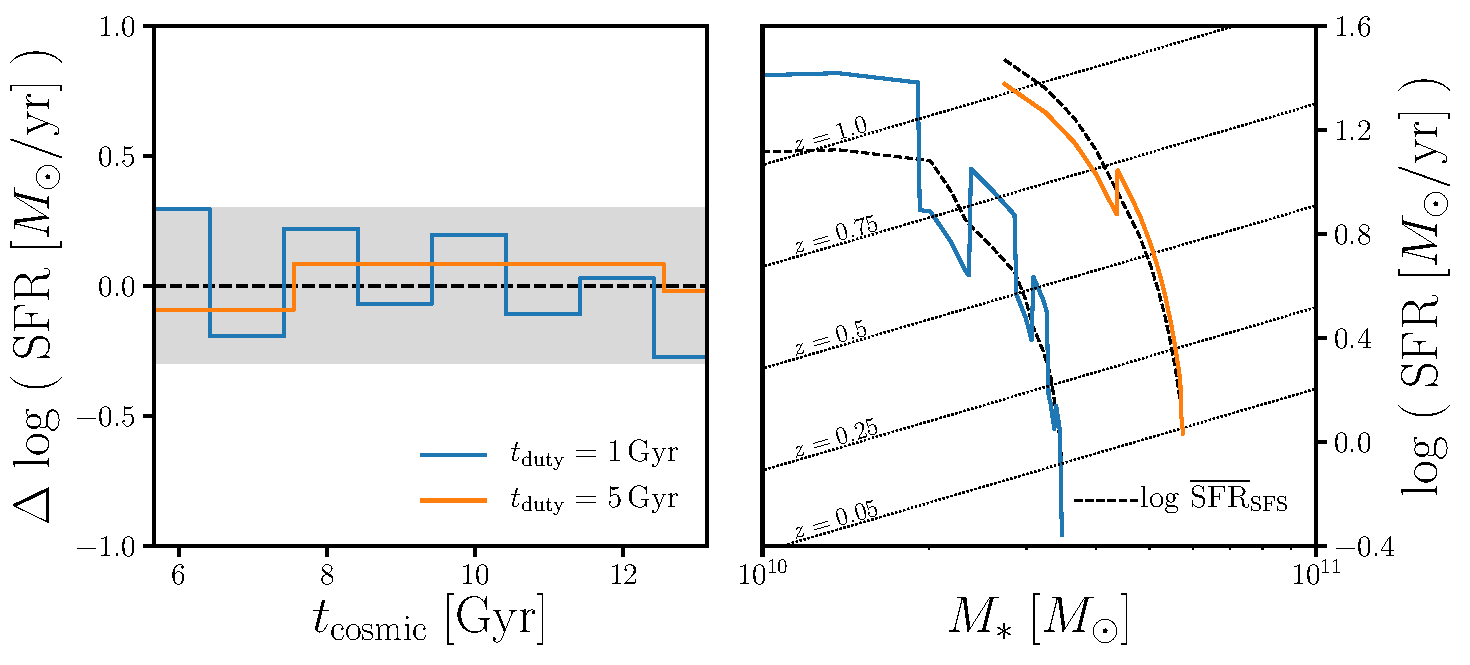
\includegraphics[width=0.9\textwidth]{figs/sfh_pedagogical.pdf}
    \caption{\emph{Left}: We illustrate the star formation duty 
    cycle prescription for $\Delta \logsfr(t)$, described 
    in Section~\ref{sec:modelevol}. The two examples we present have
    $t_\mathrm{duty} = 0.5$ Gyr (blue) and $5$ Gyr (orange). The star 
    formation duty cycle $\Delta \logsfr(t)$ combined with Eq.~\ref{eq:logsfr_sf}, 
    describe the SFHs of the star-forming central galaxies in our model. 
    \emph{Right}: We present the SFR and $M_*$ evolutions of two SF central 
    galaxies in our model with $t_\mathrm{duty} = 0.5$ Gyr (blue) and $5$ 
    Gyr (orange). The $\Delta \logsfr(t)$ for these galaxies correspond 
    to the left panel and can be seen with respect to the $\musfms(M_*, t)$ 
    plotted in black. For reference, we include the $\musfms(M_*)$ (dotted 
    lines) at various redshifts between $z = 1$ to $0.05$.} \label{fig:sfh_model}
\end{center}
\end{figure}
%%%%%%%%%%%%%%%%%%%%%%%%%%%%%%%%%%%%%


%%%%%%%%%%%%%%%%%%%%%%%%%%%%%%%%%%%%%
% Figure 5 
%%%%%%%%%%%%%%%%%%%%%%%%%%%%%%%%%%%%%
\begin{figure}
\begin{center}
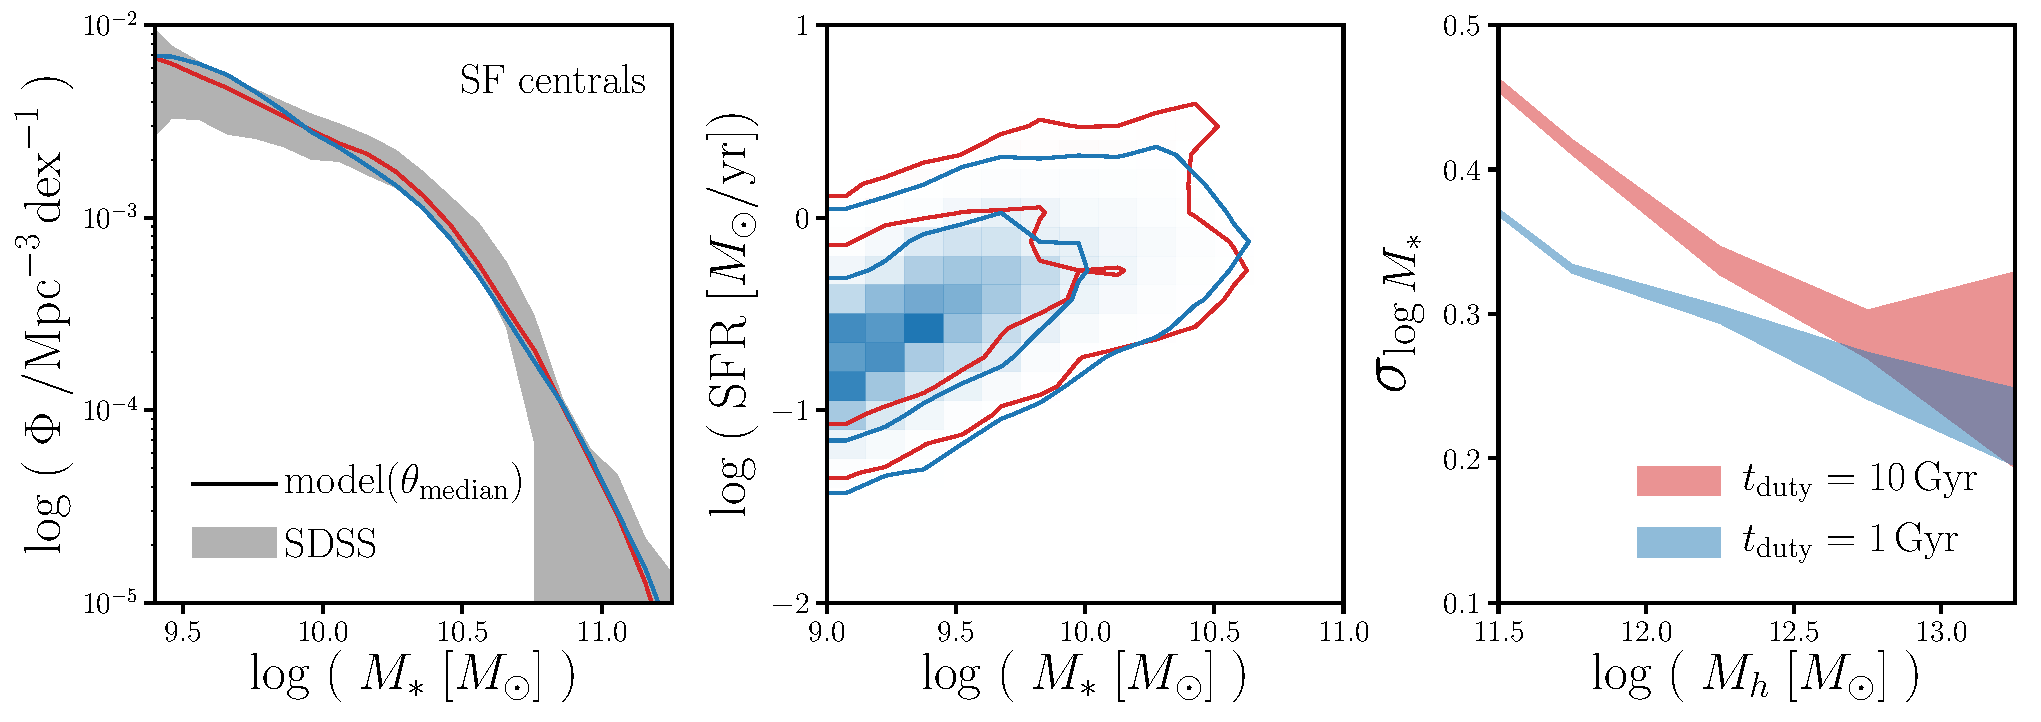
\includegraphics[width=0.9\textwidth]{figs/qaplot_abc.pdf}
\caption{}
\label{fig:abc_demo}
\end{center}
\end{figure}
%%%%%%%%%%%%%%%%%%%%%%%%%%%%%%%%%%%%%

\subsection{Evolving along the Main Sequence} \label{sec:modelevol} 
The tight correlation between the SFRs and stellar masses of SF 
galaxies (the so-called SFS) has been observed to span over four 
orders of magnitude in stellar mass and extends beyond the local 
universe out to $z > 2$ 
(\emph{e.g.}~\citealt{noeske2007,daddi2007,elbaz2007,salim2007,santini2009,karim2011,whitaker2012,moustakas2013,lee2015}; see also references in \citealt{speagle2014}). 
Even in hydrodynamic simulations and semi-analytic models, we find 
well defined SFSs (see \hahngmm and references therein). The SFRs 
of galaxies on the SFS, for a given stellar mass follow a log-normal 
distribution with a roughly constant scatter ($\sim0.3\,\mathrm{dex}$ 
in observations).  %In bins of $\mathrm{log}\,M_*$, the SFRs of galaxies on the SFS are observed to follow a log-normal distribution with a roughly constant scatter of $0.3\,\mathrm{dex}$. 
Given its persistence in the local Universe, the SFS provides a 
anchoring relationship to characterize the SFRs and $M_*$s of SF 
galaxies throughout $z < 1$. More specifically, \emph{we can characterize 
the star formation histories (SFHs) of our SF centrals with respect 
to the mean $\logsfr$ of the SFS} (Eq.~\ref{eq:logsfr_ms}):
\beq \label{eq:logsfr_sf} 
\logsfr(M_*, t) = \log\,\overline{\mathrm{SFR}}_\mathrm{MS}(M_*, t) + \Delta \logsfr(t).
\eeq
Since SFHs determine the $M_*$ growth of galaxies, $\Delta \logsfr$s
in our model dictate the SFHs and $M_*$ evolution of SF centrals. 
Below, we describe the prescription for our fiducial $\Delta \logsfr(t)$.

One naive example for $\Delta \logsfr(t)$ would be to keep 
$\Delta \logsfr$ fixed from the initial offsets from the $\musfms$
in the initial SFRs of our SF central galaxies at $z\sim1$.
%In the previous section, we selected the initial SFRs of our SF centrals by sampling the log-normal distribution about the mean SFS at $z \sim 1$.  One simple prescription for $\Delta \logsfr(t)$, would be to fix $\Delta \logsfr$ based on the initial offsets from the $\musfms$.
SF centrals with higher than average initial SFRs continue evolving 
above the average SFS, while SF centrals with lower than average 
initial SFRs continue evolving below the average SFS. In addition to 
the fact that such a SFH cannot reproduce observations, we will later 
demonstrate, we do not find such a SFH in SF galaxies of hydrodynamic 
simulations such as Illustris~\cite{vogelsberger2014,genel2014}. 
%the observed scatter in the stellar mass of SF centrals at fixed halo mass. % With such SFHs, as we demonstrate later in detail, the scatter in stellar mass of the SF centrals at fixed halo mass diverges substantially with cosmic time. 
%Furthermore, in hydrodynamic simulations such as Illustris~\cite{vogelsberger2014,genel2014}, we find that $\Delta \logsfr(t)$ of SF galaxies do not remain constant.
In Figure~\ref{fig:illsfh}, we plot $\Delta \logsfr$s of SF galaxies 
in Illustris as a function of cosmic time. These galaxies have stellar 
masses within $10^{10.5}-10^{10.6}M_\odot$ at $z=0$. At each simultation 
output, we derive $\musfms$ using the same \hahngmm fitting method as in
Section~\ref{sec:sfcen} and use it to calculate $\Delta \logsfr$ 
(Eq.~\ref{eq:logsfr_sf}). As the $\Delta \logsfr$s highlighted in color 
illustrate, the $\Delta \logsfr(t)$s of SF galaxies do not remain constant, 
but rather vary about the SFS. 
%Rather than remaining constant, Figure~\ref{fig:illsfh} illustrates that the $\Delta \logsfr(t)$s stochastically vary about SFS. 

Motivated by the $\Delta \logsfr(t)$ of Illustris galaxies, we introduce 
varability in the SFHs of our SF centrals in the form of a ``\emph{star 
formation duty cycle}''. We parameterize $\Delta \logsfr$ to flucutate about 
the mean SFS on some duty cycle timescale $t_\mathrm{duty}$ with amplitude
randomly sampled from a log-normal distribution with $0.3\,\mathrm{dex}$ 
scatter at every $t_\mathrm{duty}$ timestep. The full SFH of the SF 
centrals follow Eq.~\ref{eq:logsfr_sf}.
%Then the SFR of a given SF central in our model will follow Eq.~\ref{eq:logsfr_sf} where at every timestep $t_\mathrm{duty}$, $\Delta \logsfr$ is randomly sampled from a log-normal distribution with $0.3\,\mathrm{dex}$ scatter. 
In the left panel of Figure~\ref{fig:sfh_model}, we 
present $\Delta \logsfr(t)$ of SF centrals with our fiducial star formation 
duty cycle prescription. The two $\Delta \logsfr(t)$s have $t_\mathrm{duty} = 0.5$ 
Gyr (blue) and $5$ Gyr (orange). The shaded region represents the observed 
$0.3\,\mathrm{dex}$ $1\sigma$ scatter of the SFS SFR. 
Although, we do not expect such a simplified model to reflect the exact 
individual SFHs of SF centrals, for the SF population it captures the 
stochasticity from gas accretion and star-bursts and allows us to measure
the timescale of such variabilities. Furthermore, this $\Delta \logsfr$ 
prescription by construction reproduces the observed log-normal SFR 
distribution of the SFS at any point in the model. 

Using our $\Delta \logsfr$ prescription, we now evolve both the SFR and $M_*$ 
of our SF centrals along the main sequence. Based on Eq.~\ref{eq:logsfr_sf},
the SFRs of our SF centrals are functions of $M_*$. Meanwhile, $M_*$ is the
integral of the SFR over time: 
\beq \label{eq:integ_mass} 
M_*(t) = f_\mathrm{retain} \int\limits_{t_0}^{t} \mathrm{SFR(M_*, t)}\,\mathrm{d}t + M_0. 
\eeq
$f_\mathrm{retain}$ here is the fraction of stellar mass that is retained after 
supernovae and stellar winds; we use $f_\mathrm{retain} = 0.6$~\citep{wetzel2013}. 
$t_0$ and $M_0$ are the initial cosmic time and stellar mass at $z \sim 1$, respectively. 
Combining Eqs.~\ref{eq:logsfr_sf} and~\ref{eq:integ_mass}, we get a different 
equation, which we solve to evolve the SFR and $M_*$ of our SF centrals.  
The right panel of Figure~\ref{fig:sfh_model} presents the SFR and $M_*$ 
evolutions for the two SF centrals with different $t_\mathrm{duty}$ from the
left panel. The behavior of the star formation duty cycle $\Delta \logsfr(t)$ 
is clearly evident with respect to $\musfms(M_*, t)$ (black solid). 
For reference, we include the $\musfms$ (dotted lines) at various redshifts 
between $z = 1$ to $0.05$. 

Now that we have a model that evolves the SFRs and $M_*$s of SF centrals, 
we can compare this model to observations. Our model is constructed using the 
SMF and SMHMR at $z = 1$ and based on the observed evolution of the SFS. 
It has two free parameters $A_z$ and $m_z$, which allow for a flexible redshift 
dependence of the SFS. At the final snapshot, $z \sim 0$, our model reproduces 
the observed SFR distribution by construction. However, we also want our model to 
reproduce the observed SMF of central galaxies in SDSS. In order to do a principled
comparison of our model to observation, we use the parameter estimation framework 
of Approximate Bayesian Computation (ABC). ABC has the advantage over standard 
approaches to parameter inference in that it does not 
require evaluating the likelihood. It relies only on a simulation of the observed 
data and a distance metric to quantify the ``closeness'' between the observed data
and simulation. Many variations of ABC has been used in astronomy and 
cosmology~\citep[\emph{e.g.}][]{cameron2012,weyant2013,ishida2015,alsing2018}. 
We use ABC in conjunction with the efficient Population Monte Carlo (PMC)
importance sampling as in~\citep{hahn2016, hahn2017}. For the priors of $A_z$ and $m_z$, 
we use uniform distributions spanning the ranges \todo{numbers} and \todo{numbers}, 
respectively. As we mentioned in Section~\ref{sec:sfcen}, the range of the prior 
were conservatively chosen to encompass the best-fit SFS from~\cite{speagle2014} 
and measurements from~\cite{moustakas2013} and~\cite{lee2015} at $z \sim 1$. 
Finally, to compare the SMF of our model to the SMF of SDSS central galaxies, 
we use the following distance metric: 
\beq
\rho_\Phi = \sum\limits_{M} \left( \frac{\Phi^\mathrm{sim}(M) - f^\mathrm{cen}(M) \Phi^\mathrm{SDSS}(M)}{\sigma_\Phi(M)}\right)^2.
\eeq
$\Phi^\mathrm{sim}(M)$ is the SMF of our model, $f^\mathrm{cen}(M)$ is the
central galaxy fraction~\cite{wetzel2013}, $\Phi^\mathrm{SDSS}(M)$ is 
the~\cite{li2009} SDSS DR7 SMF, and $\sigma_\Phi(M)$ is the SMF uncertainty 
derived using mock catalogs from~\cite{li2009}. For the rest of our ABC-PMC 
implementation, we strictly follow the implementation of \cite{hahn2017b} 
and~\cite{hahn2017a}. We refer reader to those papers for further details.

In Figure~\ref{fig:abc_demo}, we present the SMFs (left), SFSs (center), and 
$\sigma_{\log\,M_*}(\mathrm{log}\,M_\mathrm{halo})$ (right) of the resulting
ABC posterior distributions of $A_z$ and $m_z$ for two models with different 
SFH prescriptions: one with no star formation duty cycle (red) and the other 
with star formation duty cycle $t_\mathrm{duty} = 1\,\mathrm{Gyr}$ (blue). 
On the left, we illustrate that the ABC posteriors successfully reproduce
the $z \sim 0$ SMF of SDSS centrals. In the center, we demonstrate how our 
models by construction, reproduce the $z\sim0$ SFS. Lastly, on the right, 
we demonstrate that different prescriptions for SFHs in our model produce significantly
different scatter in $\log\,M_*$ for a given $\log\,M_\mathrm{halo}$ --- 
\emph{i.e.} scatter in the SMHMR. Since there are observation constraints on 
the SMHMR, this means that we can them to better understand and constrain 
the SFHs of star forming galaxies. 

%%%%%%%%%%%%%%%%%%%%%%%%%%%%%%%%%%%%%
% Figure 5 
%%%%%%%%%%%%%%%%%%%%%%%%%%%%%%%%%%%%%
\begin{figure}
\begin{center}
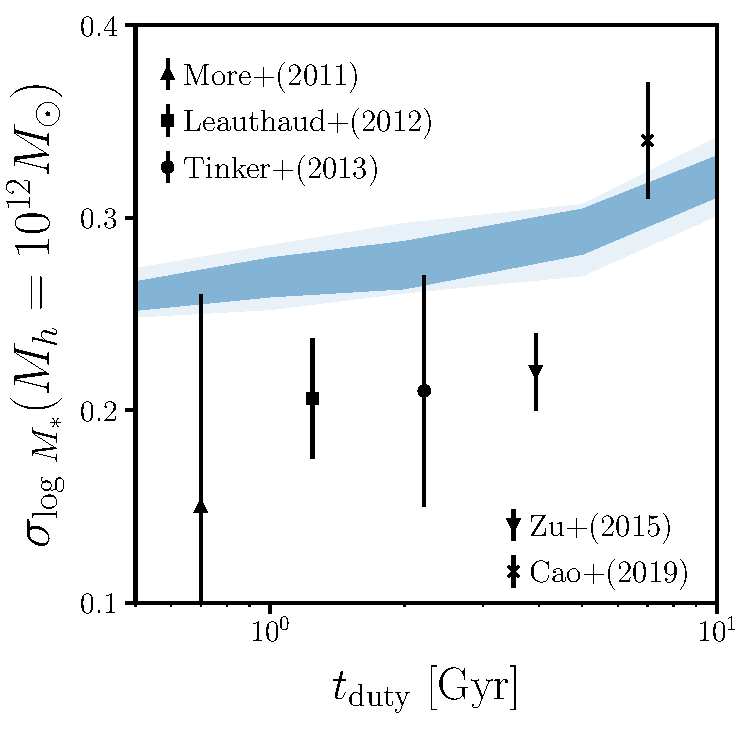
\includegraphics[width=0.9\textwidth]{figs/SHMRscatter_tduty.pdf}
\caption{}
\label{fig:sigMstar_duty}
\end{center}
\end{figure}
%%%%%%%%%%%%%%%%%%%%%%%%%%%%%%%%%%%%%

\section{Results}
\subsection{The Star Formation Duty Cycle}
Our model, described in the previous section, tracks the SFR and $M_*$ 
evolutions of SF central galaxies. After using ABC, 

%Now that we have a model that evolves the SFRs and $M_*$s of SF centrals, we can compare this model to observations. Our model is constructed using the SMF and SMHMR at $z = 1$ and based on the observed evolution of the SFS.  It has two free parameters $A_z$ and $m_z$, which allow for a flexible redshift dependence of the SFS. At the final snapshot, $z \sim 0$, our model reproduces the observed SFR distribution by construction. However, we also want our model to 


In the previous section we describe our model constructed from blah with different
prescriptions for the star formation histories of star-forming galaxies. As the 
right panel of Figure~\ref{fig:abc_demo} demonstrates, different prescriptions for 
the star-forming galaxy star formation predicts different $\sigma_{\log\,M_*}$ 

\bitem
\item Explain how the posteriors from ABC ultimately marginalize over the parameters that incorporate the 
    uncertainty in the SFS 
\item As Figure~\ref{fig:abc_demo} already demonstrates, different prescriptions lead to different scatter in the SMHMR. 
\item No duty cycle model obviously ruled out 
\item In Figure~\ref{fig:sigMstar_duty} we present the scatter in $\sigma_{\log\,M_*}$
\item We find that by decreasing the timescale of stochasticity on a simple SFH model that traces the overall 
SFS evolution does in fact decrease the scatter seen in the SMHMR. However, even with timescales less
than XXXX, we cannot reproduce observations. Ultimately to reproduce observations, we need to add in 
assembly bias. 
\eitem

Figure~\ref{fig:sigMstar_duty} 

%%%%%%%%%%%%%%%%%%%%%%%%%%%%%%%%%%%%%
% Figure 6 
%%%%%%%%%%%%%%%%%%%%%%%%%%%%%%%%%%%%%
\begin{figure}
\begin{center}
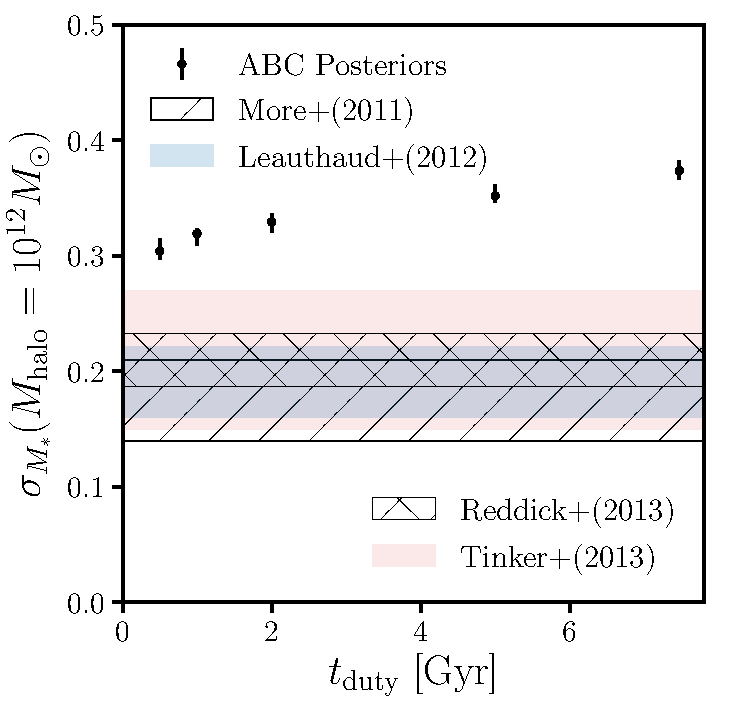
\includegraphics[width=0.5\textwidth]{figs/sigMstar_tduty.pdf}
\caption{}
\label{fig:abc_demo}
\end{center}
\end{figure}
%%%%%%%%%%%%%%%%%%%%%%%%%%%%%%%%%%%%%

\subsection{The need for a galaxy assembly bias}
\bitem
\item discuss how $t_{duty}$ is not enough to be consistent with $\sigma_{M_*}$. 
\item first clarify what you mean by galaxy assembly bias 
\item discuss implementation of galaxy assembly bias
\item Figure (pedagogical) of dlogSFR versus dMh dt for different correlation amounts 
\item Figure of different tdelay and dtabias 
\item Figure of sigma M star as a function of duty cycle and realistic dt abias and t delay 
\eitem

\section{Discussion} \label{sec:discussion}
\subsection{Rethinking the Main Sequence?}
\bitem 
\item Test the SMHMR for Louis's SFHs 
\eitem 

\section{Summary} \label{sec:summary}


\appendix
\section{$z \sim 1$ observations} \label{app:z1}
Much of the results presented in this paper are based on comparison 
between our model and observations at $z \sim 0.$. Our model is initalized 
at $z \sim 1$. Therefore, in this section we test some of the choices 
we make in our intializations. 

\bitem
\item Test impact of $z \sim 1$ SMF
\item Test impact of $z \sim 1$ $\sigma_{\log M_*}$ 
\eitem

%%%%%%%%%%%%%%%%%%%%%%%%%%%%%%%%%%%%%%%%%%%%%%%%%%%%%%%%%%%%%%%
% Acknowledgements
%%%%%%%%%%%%%%%%%%%%%%%%%%%%%%%%%%%%%%%%%%%%%%%%%%%%%%%%%%%%%%%
\section*{Acknowledgements}
It's a pleasure to thank 
    Louis Abramson, 
    Shy Genel, 
    \todo{more acknowledgements} 
for valueable discussions. 

\bibliographystyle{yahapj}
\bibliography{centralMS}
\end{document}
